\documentclass[12pt,a4paper]{article}
\usepackage{amsmath,amssymb,mathrsfs,tikz,times,pifont}
\usepackage{enumitem}
\newcommand\circitem[1]{%
\tikz[baseline=(char.base)]{
\node[circle,draw=gray, fill=red!55,
minimum size=1.2em,inner sep=0] (char) {#1};}}
\newcommand\boxitem[1]{%
\tikz[baseline=(char.base)]{
\node[fill=cyan,
minimum size=1.2em,inner sep=0] (char) {#1};}}
\setlist[enumerate,1]{label=\protect\circitem{\arabic*}}
\setlist[enumerate,2]{label=\protect\boxitem{\alph*}}
%%%::::::by chnini ameur :::::::%%%
\everymath{\displaystyle}
\usepackage[left=1cm,right=1cm,top=1cm,bottom=1.7cm]{geometry}
\usepackage[colorlinks=true, linkcolor=blue, urlcolor=blue, citecolor=blue]{hyperref}
\usepackage{array,multirow}
\usepackage[most]{tcolorbox}
\usepackage{varwidth}
\usepackage{float} %pour utiliser l'option [H] qui force l'image à apparaître exactement à l'endroit où elle est placée dans le code.
\tcbuselibrary{skins,hooks}
\usetikzlibrary{patterns}
%%%::::::by chnini ameur :::::::%%%
\newtcolorbox{exa}[2][]{enhanced,breakable,before skip=2mm,after skip=5mm,
colback=yellow!20!white,colframe=black!20!blue,boxrule=0.5mm,
attach boxed title to top left ={xshift=0.6cm,yshift*=1mm-\tcboxedtitleheight},
fonttitle=\bfseries,
title={#2},#1,
% varwidth boxed title*=-3cm,
boxed title style={frame code={
\path[fill=tcbcolback!30!black]
([yshift=-1mm,xshift=-1mm]frame.north west)
arc[start angle=0,end angle=180,radius=1mm]
([yshift=-1mm,xshift=1mm]frame.north east)
arc[start angle=180,end angle=0,radius=1mm];
\path[left color=tcbcolback!60!black,right color = tcbcolback!60!black,
middle color = tcbcolback!80!black]
([xshift=-2mm]frame.north west) -- ([xshift=2mm]frame.north east)
[rounded corners=1mm]-- ([xshift=1mm,yshift=-1mm]frame.north east)
-- (frame.south east) -- (frame.south west)
-- ([xshift=-1mm,yshift=-1mm]frame.north west)
[sharp corners]-- cycle;
},interior engine=empty,
},interior style={top color=yellow!5}}
%%%%%%%%%%%%%%%%%%%%%%%

\usepackage{fancyhdr}
\usepackage{eso-pic}         % Pour ajouter des éléments en arrière-plan
% Commande pour ajouter du texte en arrière-plan
\usepackage{tkz-tab}
\AddToShipoutPicture{
    \AtTextCenter{%
        \makebox[0pt]{\rotatebox{80}{\textcolor[gray]{0.7}{\fontsize{5cm}{5cm}\selectfont PGB}}}
    }
}
\usepackage{lastpage}
\fancyhf{}
\pagestyle{fancy}
\renewcommand{\footrulewidth}{1pt}
\renewcommand{\headrulewidth}{0pt}
\renewcommand{\footruleskip}{10pt}
\fancyfoot[R]{
\color{blue}\ding{45}\ \textbf{2024}
}
\fancyfoot[L]{
\color{blue}\ding{45}\ \textbf{Prof:M. BA}
}
\cfoot{\bf
\thepage /
\pageref{LastPage}}
\begin{document}
\renewcommand{\arraystretch}{1.5}
\renewcommand{\arrayrulewidth}{1.2pt}
\begin{tikzpicture}[overlay,remember picture]
\node[draw=blue,line width=1.2pt,fill=purple,text=blue,inner sep=3mm,rounded corners,pattern=dots]at ([yshift=-2.5cm]current page.north) {\begingroup\setlength{\fboxsep}{0pt}\colorbox{white}{\begin{tabular}{|*1{>{\centering \arraybackslash}p{0.28\textwidth}} |*2{>{\centering \arraybackslash}p{0.2\textwidth}|} *1{>{\centering \arraybackslash}p{0.19\textwidth}|} }
\hline
\multicolumn{3}{|c|}{$\diamond$$\diamond$$\diamond$\ \textbf{Lycée de Dindéfélo}\ $\diamond$$\diamond$$\diamond$ }& \textbf{A.S. : 2024/2025} \\ \hline
\textbf{Matière: Mathématiques}& \textbf{Niveau : T}\textbf{S2} &\textbf{Date: 09/12/2024} & \textbf{Durée : 4 heures} \\ \hline
\multicolumn{4}{|c|}{\parbox[c]{10cm}{\begin{center}
\textbf{{\Large\sffamily Correction du devoir n$ ^{\circ} $ 1 Du 1$ ^\text{\bf er} $ Semestre}}
\end{center}}} \\ \hline
\end{tabular}}\endgroup};
\end{tikzpicture}
\vspace{3cm}

\section*{\underline{Exercice 1 :} $1,5$ points}

\begin{enumerate}

\item Déterminons les racines cubiques de l'unité.

Résolvons pour cela $z^3 = 1$, $z \in \mathbb{C}$ :

\[
z^3 = 1 \implies z^3 = e^{i(0+2k\pi)}, \quad k \in \mathbb{Z}.
\]

\[
z = e^{i\frac{(0+2k\pi)}{3}}, \quad k = 0, 1, 2.
\]

- Pour $k = 0$, $z = e^{i0} = 1$, donc $z_0 = 1$.

- Pour $k = 1$, $z = e^{i\frac{2\pi}{3}} = \cos\frac{2\pi}{3} + i\sin\frac{2\pi}{3} = -\frac{1}{2} + i\frac{\sqrt{3}}{2}$, donc $z_1 = -\frac{1}{2} + i\frac{\sqrt{3}}{2}$.

- Pour $k = 2$, $z = e^{i\frac{4\pi}{3}} = \cos\frac{4\pi}{3} + i\sin\frac{4\pi}{3} = -\frac{1}{2} - i\frac{\sqrt{3}}{2}$, donc $z_2 = -\frac{1}{2} - i\frac{\sqrt{3}}{2}$.

Ainsi, l'ensemble des solutions est :

\[
S_{\mathbb{C}} = \left\{ 1, -\frac{1}{2} + i\frac{\sqrt{3}}{2}, -\frac{1}{2} - i\frac{\sqrt{3}}{2} \right\}.
\]

\item Interprétation

\begin{itemize}
    \item $\text{arg}(z_B - z_A) = (\overrightarrow{OI}, \overrightarrow{AB}) \, [2\pi]$
    
    Géométriquement, $\text{arg}(z_B - z_A)$ est l'angle $\widehat{(\overrightarrow{OI}, \overrightarrow{AB})}$ formé par le vecteur $\overrightarrow{AB}$ avec l'axe réel du plan complexe $(O, \overrightarrow{OI})$.

    \item $\text{arg}\left(\frac{z_B - z_C}{z_B - z_A}\right) = (\overrightarrow{AB}, \overrightarrow{CD}) \, [2\pi]$
    
    Géométriquement, $\text{arg}\left(\frac{z_B - z_C}{z_B - z_A}\right)$ est l'angle $\widehat{(\overrightarrow{AB}, \overrightarrow{CD})}$ que forment les vecteurs $\overrightarrow{AB}$ et $\overrightarrow{CD}$.
\end{itemize}

\item $f(x) = \sqrt{x}$, appliquons l'IAF

Appliquons l'IAF (Inégalité des Accroissements Finis) sur $[t, t+1]$.

\boxed{
\begin{aligned}
&\textbf{Théorème des Inégalités des Accroissements Finis (TI-AF 1)} \\
&\text{Soit } f \text{ une fonction définie sur un intervalle } [a, b]. \\
&\text{Hypothèses :} \\
&\quad 1) , f \text{ est continue sur } [a, b]. \\
&\quad 2) , f \text{ est dérivable sur } ]a, b[. \\
&\quad 3) , \text{Il existe deux réels } m \text{ et } M \text{ tels que, pour tout } x \in ]a, b[, m \leq f'(x) \leq M. \\
&\text{Conclusion :} \\
&\quad m(b - a) \leq f(b) - f(a) \leq M(b - a). \\
&\textbf{Théorème des Inégalités des Accroissements Finis (TI-AF 2)} \\
&\text{Soit } f \text{ une fonction définie sur un intervalle } [a, b]. \\
&\text{Hypothèses :} \\
&\quad 1) , f \text{ est continue sur } [a, b]. \\
&\quad 2) , f \text{ est dérivable sur } ]a, b[. \\
&\quad 3) , \text{Il existe un réel } m \geq 0 \text{ tel que, pour tout } x \in ]a, b[, |f'(x)| \leq m. \\
&\text{Conclusion :} \\
&\quad |f(b) - f(a)| \leq m|b - a|.
\end{aligned}
}


\textbf{Applications} $t > 0$

\begin{itemize}
    \item $f$ est continue sur $[t, t+1]$.
    \item $f$ est dérivable sur $]t, t+1[$ et pour tout,
\[
    \forall x \in ]t, t+1[, \quad f'(x) = \frac{1}{2\sqrt{x}}.
\]
\end{itemize}

Comme $x \in ]t, t+1[$, alors $t < x < t+1$. Ainsi, 
\[
\frac{1}{2\sqrt{t+1}} < \frac{1}{2\sqrt{x}} < \frac{1}{2\sqrt{t}}.
\]

D'où :
\[
\frac{1}{2\sqrt{t+1}} < f'(x) < \frac{1}{2\sqrt{t}}.
\]

En appliquant l'inégalité des accroissements finis (IAF), nous avons :
\[
\frac{1}{2\sqrt{t+1}}(t+1-t) < f(t+1) - f(t) < \frac{1}{2\sqrt{t}}(t+1-t).
\]

Cela donne :
\[
\frac{1}{2\sqrt{t+1}} < f(t+1) - f(t) < \frac{1}{2\sqrt{t}}.
\]

\end{enumerate}

\section*{\underline{Exercice 2 :} 8,5 points}

\subsection*{ Partie A}
\begin{enumerate}
\item Montrons que $P$ admet une unique racine réelle.

Soit $z_0 = a \in \mathbb{R}$ tel que $P(z_0) = 0$.

\[
P(z) = z^3 + (-5 + 2i)z^2 + (7 - 7i)z - 2 + 6i
\]

\[
P(z_0) = 0 \implies a^3 + (-5 + 2i)a^2 + (7 - 7i)a - 2 + 6i = 0
\]

\[
\implies a^3 - 5a^2 + 7a - 2 + i\big(2a^2 - 7a + 6\big) = 0
\]

En séparant les parties réelle et imaginaire :
\[
\begin{cases}
a^3 - 5a^2 + 7a - 2 = 0 \quad (1) \\
2a^2 - 7a + 6 = 0 \quad (2)
\end{cases}
\]

L'équation (2) est plus facile à résoudre.

Résolution de (2)

\[
2a^2 - 7a + 6 = 0
\]

Calculons le discriminant :
\[
\Delta = 7^2 - 4 \times 2 \times 6 = 49 - 48 = 1.
\]

Les solutions sont :
\[
a_1 = \frac{-(-7) - \sqrt{\Delta}}{2 \times 2} = \frac{7 - 1}{4} = \frac{6}{4} = \frac{3}{2},
\]
\[
a_2 = \frac{-(-7) + \sqrt{\Delta}}{2 \times 2} = \frac{7 + 1}{4} = \frac{8}{4} = 2.
\]

La racine de (2) qui vérifie (1) est la racine de $P(z)$.

Vérification pour $a = \frac{3}{2}$

\underline{Substituons $a = \frac{3}{2}$ dans (1) :}
\begin{align*}
a^3 - 5a^2 + 7a - 2 &= \left(\frac{3}{2}\right)^3 - 5\left(\frac{3}{2}\right)^2 + 7\left(\frac{3}{2}\right) - 2\\
										&=\frac{27}{8} - 5 \times \frac{9}{4} + \frac{21}{2} - 2\\
										&=\frac{27}{8} - \frac{45}{8} + \frac{84}{8} - \frac{16}{8}\\
										&=\frac{27 - 45 + 84 - 16}{8}\\
										&= \frac{111 - 106}{8} = \frac{5}{8} \neq 0
\end{align*}

Donc, $a = \frac{3}{2}$ n'est pas solution.

\underline{Vérification pour $a = 2$}

Substituons $a = 2$ dans (1) :

\begin{align*}
a^3 - 5a^2 + 7a - 2 &= 2^3 - 5(2^2) + 7(2) - 2\\
										&=8 - 20 + 14 - 2\\
										&=0
\end{align*}

Donc, $a = 2$ est une solution.

\[
z_0 = 2.
\]

\item Factorisons $P(z)$

Utilisons la méthode de la division synthétique pour factoriser $P(z)$. Le tableau est donné ci-dessous :

\[
\begin{array}{|c|c|c|c|c|}
\hline
\text{ } & 1 & -5+2i & 7-7i & 2+6i \\ 
\hline
2 & \downarrow & 2 & -6+i & 2-6i \\ 
\hline
\text{ } & 1 & -3+2i & 1-3i & 0 \\ 
\hline
\end{array}
\]

Ainsi, nous avons :
\[
P(z) = (z - 2)\big(z^2 + (-3+2i)z + 1-3i\big).
\]

\item Résolvons $P(z) = 0$

\[
P(z) = 0 \implies z = 2 \quad \text{ou} \quad z^2 + (-3+2i)z + 1-3i = 0.
\]

\begin{align*}
\Delta &= (-3+2i)^2 - 4(1)(1-3i)\\
 			 &= 9 - 12i - 4 + 12i\\
	     &= 5
\end{align*}

\[
z_{1} = \frac{3-\sqrt{5}}{2}-i, z_{2} = \frac{3+\sqrt{5}}{2}-i
\]

\[
S = \left\{ 2, \frac{3-\sqrt{5}}{2}-i, \frac{3+\sqrt{5}}{2}-i \right\}.
\]

\end{enumerate}
\subsection*{ Partie B}

\begin{enumerate}
\item Représentation

\begin{center}
\begin{tikzpicture}[scale=2]

    % Axes avec origine décalée à gauche
    \draw[->] (-1,0) -- (3.5,0) node[below] {\( \text{Re} \)};
    \draw[->] (0,-1.5) -- (0,2.5) node[left] {\( \text{Im} \)};
    
    % Cercle unité pour illustration de l'angle
    \draw[dashed, gray] (0,0) circle(1);

    % Points
    \filldraw[red] (2,-1) circle(2pt) node[below right] {\( A(2,-1) \)};
    \filldraw[red] (2,0) circle(2pt) node[above right] {\( B(2) \)};
    \filldraw[red] (1,-1) circle(2pt) node[below left] {\( C(1,-1) \)};
    \filldraw[red] (1,0) circle(2pt) node[above left] {\( D(1) \)};
    
    % Lignes de connexion
    \draw[thick, dashed, blue] (2,-1) -- (2,0) -- (1,0) -- (1,-1) -- cycle;
    
    % Angle de π/3
    \draw[thick] (0.7,0) arc[start angle=0, end angle=60, radius=0.7];
    \node at (0.9,0.3) {\(\frac{\pi}{3}\)};
    
    % Vecteur illustrant un nombre complexe sur le cercle
    \draw[thick, ->] (0,0) -- (cos{60},sin{60});
    
\end{tikzpicture}
\end{center}

\item Écriture exponentielle de $z_C$ et $z_E$

\underline{Pour $z_C$ :}

\begin{align*}
z_C &= 1 - i\\
		&= \sqrt{2} \left(\cos\left(-\frac{\pi}{4}\right) + i\sin\left(-\frac{\pi}{4}\right)\right)\\
		&= \sqrt{2} e^{-i\pi/4}\\
\end{align*}
 \[ \boxed{ z_C=\sqrt{2} e^{-i\pi/4}} \]
\underline{Pour $z_E$ :}

\begin{align*}
z_E &= 1 + i\sqrt{3}\\
	  &= 2 \left(\frac{1}{2} + i\frac{\sqrt{3}}{2}\right)\\
		&= 2 \left(\cos\left(\frac{\pi}{3}\right) + i\sin\left(\frac{\pi}{3}\right)\right)\\
		&= 2 e^{i\pi/3}
\end{align*}

Donc :
\[ \boxed{z_E = 2 e^{i\pi/3}} \]

\item 3. Plaçons exactement le point $E$

\[
z_E = 2 e^{i\pi/3}.
\]

\item Écriture algébrique de $z_E^8$

\begin{align*}
z_E = 2 e^{i\pi/3} &\implies z_E^8 = 2^8 e^{8i\pi/3}\\
                   &\implies z_E^8=2^8 \left[\cos\left(\frac{2\times 3\pi}{3}+\frac{2\pi}{3}\right) + i\sin\left(\frac{2\times 3\pi}{3}+\frac{2\pi}{3}\right)\right]\\
										&\implies z_E^8=\left[\cos\left(2\pi+\frac{2\pi}{3}\right) + i\sin\left(2\pi+\frac{2\pi}{3}\right)\right]\\
										&\implies z_E^8 = 2^8 \left(-\frac{1}{2} + i\frac{\sqrt{3}}{2}\right)
\end{align*}

\[
\boxed{z_E^8 = 2^8 \left(-\frac{1}{2} + i\frac{\sqrt{3}}{2}\right)}.
\]

\item 5. Calculons les affixes de $I$ et $J$

On a : $ I = \text{bar}\{(A,1); (C,-2)\} $
\begin{align*}
I = \text{bar}\{(A,1); (C,-2)\} &\implies \overrightarrow{AI} = \frac{-2}{1-2} \overrightarrow{AC}\\
                                &\implies \overrightarrow{AI} = 2 \overrightarrow{AC}\\
                                &\implies Z_I - Z_A = 2 (Z_C - Z_A)\\
                                &\implies Z_I - Z_A = 2Z_C - 2Z_A\\
                                &\implies Z_I = 2Z_C - Z_A\\
                                &\implies Z_I = 2 (1 - i) - (2 - i)\\
                                &\implies Z_I = 2 - 2i - 2 + i\\
                                &\implies Z_I = -i.
\end{align*}

\[
\boxed{Z_I = -i}
\]


On a: $ J = \text{bar}\{(A,1); (C,2)\} $

\begin{align*}
\text{Donc } J = \text{bar}\{(A,1); (C,2)\} &\implies \overrightarrow{AJ} = \frac{2}{1+2} \overrightarrow{AC}\\
															 &\implies Z_J - Z_A = \frac{2}{3} Z_C - \frac{2}{3} Z_A\\
                               &\implies Z_J = \frac{2}{3} Z_C + \frac{1}{3} Z_A\\
                               &\implies Z_J = \frac{2}{3} (1 - i) + \frac{1}{3} (2 - i)\\
                               &\implies Z_J = \frac{2}{3} + \frac{2}{3} (-i) + \frac{2}{3} - \frac{i}{3}\\
                               &\implies Z_J = \frac{4}{3} - i
\end{align*}

\[
\boxed{Z_J = \frac{4}{3} - i}
\]

\item Donner un module et un argument de $\frac{Z_B - Z_A}{Z_C - Z_A}$

\begin{align*}
\frac{Z_B - Z_A}{Z_C - Z_A} &= \frac{2 - (2 - i)}{1 - i - (2 - i)}\\
														&= \frac{i}{-1}\\
														&= i
\end{align*}

\[
\text{Donc } \boxed{\frac{Z_B - Z_A}{Z_C - Z_A} = i}
\]

\textbf{Module}

\[
\left| \frac{Z_B - Z_A}{Z_C - Z_A} \right| = |i| = 1
\]

\textbf{Un Argument}

\[
\arg\left( \frac{Z_B - Z_A}{Z_C - Z_A} \right) = \frac{\pi}{2}
\]

\item Nature de $ABC$

\[
\begin{cases}
\left| \frac{Z_B - Z_A}{Z_C - Z_A} \right| = 1\\
\arg\left( \frac{Z_B - Z_A}{Z_C - Z_A} \right) = \frac{\pi}{2} 
\end{cases}\implies
\begin{cases}
AB = AC\\
\left(\overrightarrow{AC},\overrightarrow{AB} \right) = \frac{\pi}{2}
\end{cases}
\]
%\left( \widehat{ACB}, \widehat{CAB} \right) = \frac{\pi}{2}
\[
\text{Donc } ABC \text{ est un triangle rectangle et isocèle en } A.
\]

\item Montrons que $A, B, C, D$ sont cocycliques

On a :

\[
BD = |Z_D - Z_B| = |1 - 2| = 1
\]

\[
DC = |Z_C - Z_D| = |i - i - 1| = 1
\]

\textbf{Conclusion} 

\[
\text{donc } AB = AC = BD = DC \quad \text{et} \quad \widehat{(AC, AB)} = \frac{\pi}{2}.
\]

\[
\text{donc } ABDC \text{ est un carré, donc il est inscrit dans un cercle } \mathcal{C}\left(\frac{z_{A}+z_{D}}{2},\frac{|z_{A}-z_{D}|}{2} \right) .
\]

\[
\text{Tel que les sommets de } ABCD \text{ appartiennent à } \mathcal{C}.
\]

\begin{align*}
\frac{z_{A}+z_{D}}{2}&=\frac{2-i+1}{2}\\
					 &=\frac{3-i}{2}\\
\end{align*}

\begin{align*}
\frac{|z_{A}-z_{D}|}{2}&=\frac{|2-i-1|}{2}\\
						&=\frac{|1-i|}{2}\\
						&=\frac{\sqrt{2}}{2}
\end{align*}

$$ \boxed{\mathcal{C}\left( \left( \frac{3-i}{2} \right) , \frac{\sqrt{2}}{2} \right)} $$

$$ \boxed{\mathcal{C} \left( \begin{pmatrix} \frac{3}{2} \\ -\frac{1}{2} \end{pmatrix}, \frac{\sqrt{2}}{2} \right)} $$
\item Forme exponentielle de $Z$ et Écriture algébrique $Z$

\begin{enumerate}
\item Forme exponentielle de $Z$
\[
Z = \frac{Z_E}{Z_C}
\]


\begin{align*}
\begin{cases}
Z_E = 2 e^{i\pi/3}\\
Z_C = \sqrt{2} e^{-i\pi/4}
\end{cases}
&\iff Z = \frac{2 e^{i\pi/3}}{\sqrt{2} e^{-i\pi/4}}\\
&\iff Z = \sqrt{2} e^{i(\pi/3 + \pi/4)}\\
&\iff Z = \sqrt{2} e^{i\frac{7\pi}{12}}
\end{align*}
\[
\boxed{Z = \sqrt{2} e^{i\frac{7\pi}{12}}}
\]

\item Les valeurs de $\cos\frac{7\pi}{12}$ et $\sin\frac{7\pi}{12}$

Écriture algébrique de $Z$
\begin{align*}
Z = \frac{Z_E}{Z_C}\iff Z &= \frac{1 + i\sqrt{3}}{1 - i}\\
  &= \frac{(1 + i\sqrt{3})(1 + i)}{(1 - i)(1 + i)}\\
 &= \frac{(1 + i\sqrt{3})(1 + i)}{2}\\
 &= \frac{1 + \sqrt{3}i + i - \sqrt{3}}{2}\\
Z &= \frac{1 - \sqrt{3}}{2} + i \frac{1 + \sqrt{3}}{2}
\end{align*}

\begin{align*}
Z &= \sqrt{2} e^{i\frac{7\pi}{12}}\\
Z &= \sqrt{2} \left[\cos\left(\frac{7\pi}{12}\right) + i\sin\left(\frac{7\pi}{12}\right)\right].
\end{align*}

\[
\text{Par identification : }\cos\left(\frac{7\pi}{12}\right) = \frac{\frac{1 - \sqrt{3}}{2}}{\sqrt{2}}, \quad \sin\left(\frac{7\pi}{12}\right) = \frac{\frac{1 + \sqrt{3}}{2}}{\sqrt{2}}.
\]

\[
\text{D'où : }\boxed{\cos\left(\frac{7\pi}{12}\right) = \frac{\sqrt{2} - \sqrt{6}}{4}, \quad \sin\left(\frac{7\pi}{12}\right) = \frac{\sqrt{2} + \sqrt{6}}{4}}.
\]
\end{enumerate}

\end{enumerate}
\subsection*{ Partie C}

Soit $f$ définie par :
$$
\begin{array}{rcl}
f : \mathbb{P} \setminus \{c(1 - i)\}&\to& \mathbb{P}\\
Z &\mapsto &\frac{Z - 2i}{Z - 1 + i}
\end{array}
$$
\begin{enumerate}
\item Expression de $OM'$ en fonction de $MA$ et $MC$
On a :
\[
Z' = \frac{Z - 2i}{Z - 1 + i}.
\]

\[
Z' = \frac{Z - (2 + i)}{Z - (1 + i)}.
\]

\[
Z' = \frac{Z_M - Z_A}{Z_M - Z_C}.
\]

\[
|Z'_M| = \left|\frac{Z_M - Z_A}{Z_M - Z_C}\right|.
\]

\[
OM' = \frac{MA}{MC}.
\]

\[
\boxed{OM' = \frac{MA}{MC}}
\]
\item Une interprétation géométrique de $\arg(Z')$

$\arg(Z')=\arg\left( \frac{Z_M - Z_A}{Z_M - Z_C} \right) = \left( \overrightarrow{CM};\overrightarrow{AM} \right) = \left( \overrightarrow{MC};\overrightarrow{MA} \right) $

Géométriquement, $\arg(Z')$ représente l'angle orienté entre les vecteurs $\overrightarrow{CM}$ et $\overrightarrow{AM}$.
\item L'ensemble des points M pour $Z'$ soit un réel non nul.
 \[
    Z' = \frac{Z_M - Z_A}{Z_M - Z_C}.
    \]

    Pour que $Z'$ soit un réel non nul, deux conditions doivent être satisfaites :
    \begin{enumerate}
        \item \( Z_M \neq Z_A \), car le numérateur ne doit pas être nul.
        \item \( Z_M \neq Z_C \), car le dénominateur ne doit pas être nul.
    \end{enumerate}

    Ensuite, pour que \( Z' \) soit un réel, l'argument de \(\frac{Z_M - Z_A}{Z_M - Z_C}\) doit être nul ou un multiple de \(\pi\),\\$\arg(Z')=\arg\left( \frac{Z_M - Z_A}{Z_M - Z_C} \right)=0[\pi]$, ce qui implique que les vecteurs \(\overrightarrow{CM}\) et \(\overrightarrow{AM}\) sont colinéaires.

    En termes géométriques, cela signifie que \( M \) appartient à la droite passant par \( A \) et \( C \), à l'exclusion des points \( A \) et \( C \).

    L'ensemble des points \( M \) est donc donné par :
    \[
    \mathcal{D} = \{M \in \mathbb{C} \mid M \in \text{droite}(A, C) \setminus \{A, C\}\}.
    \]
\item Donner et construire l'ensemble des points M tel que \( |Z'|=2 \)
\[
|Z'_M| = \left|\frac{Z_M - Z_A}{Z_M - Z_C}\right|=OM = \frac{MA}{MC}.
\]

\begin{align*}
MA =2MC &\implies (MA)^{2} =(2MC)^{2}\\
				&\implies (MA)^{2} -(2MC)^{2}=0\\
				&\implies (\overrightarrow{MA} - 2\overrightarrow{MC}).(\overrightarrow{MA} + 2\overrightarrow{MC}) = 0\\
\text{Or }  I = \text{bar}\{(A,1); (C,-2)\} \text{ et } J = \text{bar}\{(A,1); (C,2)\}\\
				&\implies (1-2)\overrightarrow{MI}.(2+1)\overrightarrow{MJ} = 0\\
				&\implies -3\overrightarrow{MI}.\overrightarrow{MJ} = 0\\
				&\implies \overrightarrow{MI}.\overrightarrow{MJ} = 0
\end{align*}

\( M \) décrit donc un cercle de centre $\frac{z_I+z_J}{2}$ et de rayon $\frac{|z_I-z_J|}{2}$

$ \frac{z_I+z_J}{2} = \frac{ -i+\left( \frac{4}{3} - i\right) }{2} $ \text{ et } $\frac{|z_I-z_J|}{2}=\frac{|-i-\left( \frac{4}{3} - i\right)|}{2} $

$ \frac{z_I+z_J}{2} = \frac{ \left( \frac{4}{3} - 2i\right) }{2} $ \text{ et } $\frac{|z_I-z_J|}{2}=\frac{|-\frac{4}{3}|}{2} $

$ \frac{z_I+z_J}{2} = \frac{ \left( \frac{4 - 6i}{3}\right) }{2} $ \text{ et } $\frac{|z_I-z_J|}{2}=\frac{4}{6} $

$ \frac{z_I+z_J}{2} = \frac{4 - 6i}{6} $ \text{ et } $\frac{|z_I-z_J|}{2}=\frac{4}{6} $

$ \frac{z_I+z_J}{2} = \frac{2 - 3i}{3} $ \text{ et } $\frac{|z_I-z_J|}{2}=\frac{4}{6} $

$ \frac{z_I+z_J}{2} = \frac{2}{3}-i $ \text{ et } $\frac{|z_I-z_J|}{2}=\frac{4}{6} $

$$ \text{Finalement : } \boxed{\mathcal{C}\left( \left( \frac{2}{3}-i \right)  ;\frac{4}{6}\right)} $$

$$ \boxed{\mathcal{C} \left( \begin{pmatrix} \frac{3}{2} \\ -1 \end{pmatrix}, \frac{4}{6} \right)} $$
\end{enumerate}

\section*{\underline{Problème :} 10 points}

\subsection*{Partie A}
Soit \( \mu(x) = x^3 + 3x - 1 \)

\begin{itemize}
    \item[a)] \textbf{Tableau de variation} :
        \begin{itemize}
            \item Domaine de définition : \( D_f = \mathbb{R} \)
            \item Limites aux bornes :
                  \begin{itemize}
                      \item En \( x \to -\infty \) : \( \lim\limits_{x \to -\infty} \mu(x) = -\infty \)
                      \item En \( x \to +\infty \) : \( \lim\limits_{x \to +\infty} \mu(x) = +\infty \)
                  \end{itemize}
            \item Variation de \( \mu \) :
                  \begin{itemize}
                      \item \( \mu \) est continue sur \( \mathbb{R} \) car c'est un polynôme.
                      \item \( \mu \) est aussi dérivable sur \( \mathbb{R} \).
                  \end{itemize}

            \item  Dérivée de \( \mu \)

                  On a : \( \mu'(x) = 3x^2 + 3 \)

            \item  Le signe de \( \mu'(x) \)

                  Résolvons \( \mu'(x) = 0 \) :

                  \( 3x^2 + 3 = 0 \)

                  \( x^2 = -1 \)

                  Comme \( x^2 = -1 \) n'a pas de solution réelle, on en déduit que :

                  \( \forall x \in \mathbb{R}, \quad \mu'(x) > 0 \)

                  Donc, \( \mu(x) \) est \textbf{strictement croissante} sur \( \mathbb{R} \).


                  \begin{center}
                      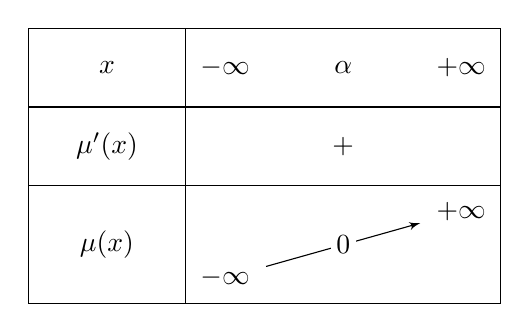
\begin{tikzpicture}
                          \tkzTabInit{$x$ /1, $\mu'(x)$ /1, $\mu(x)$ /1.5} {$-\infty$ , $+\infty$}
                          \tkzTabLine{, +,}
                          \tkzTabVar{-/$-\infty$, +/ $+\infty$}
                          \tkzTabVal{1}{2}{0.5}{$\alpha$}{0} % On place 0, son antécédent est pi / 2.
                      \end{tikzpicture}
                  \end{center}

        \end{itemize}
    \item[b)] Montrons que \( \mu(x) = 0 \) admet une unique solution dans \( ]0,1[ \)

        \textbf{Existence}

        \( \mu(0) = -1 \) et \( \mu(1) = 3 \)

        Comme \( \mu(0) \times \mu(1) < 0 \), donc \( \mu(x) = 0 \) admet une solution dans \( ]0,1[ \).

        \textbf{Unicité}

        \( \mu \) est continue et strictement croissante sur \( \mathbb{R} \), donc sur \( ]0,1[ \), \( \mu(x) = 0 \) admet une unique solution dans \( ]0,1[ \).

    \item [c)] Un encadrement de \( \alpha \) à \( 10^{-1} \) près

          \textbf{Par la méthode de balayage}

          \begin{center}
              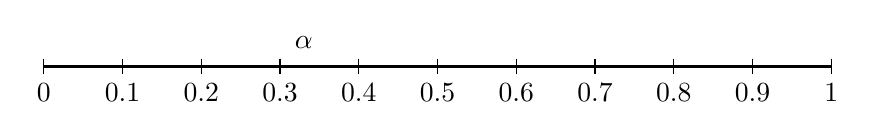
\begin{tikzpicture}
                  % Axe horizontal
                  \draw[thick] (0,0) -- (10,0);

                  % Graduations
                  \foreach \x/\val in {0/0, 1/0.1, 2/0.2, 3/0.3, 4/0.4, 5/0.5, 6/0.6, 7/0.7, 8/0.8, 9/0.9, 10/1} {
                          \draw (\x,0.1) -- (\x,-0.1) node[below] {\val};
                      }

                  % Position de alpha
                  \node[above] at (3.3,0.1) {\(\alpha\)};
              \end{tikzpicture}
          \end{center}

          \[ 0.3 \leq \alpha \leq 0.4 \]

    \item [d)] Le signe de \( \mu(x) - 1 \) pour \( \mathbb{R} \)

          \[
              \mu(x) - 1 \text{ et } \mu(x) \text{ ont les mêmes variations et mêmes limites en } -\infty \text{ et } +\infty.
          \]

          Il existe un \( \beta \) tel que  $\mu(\beta)-1 = 0$

          \begin{center}
              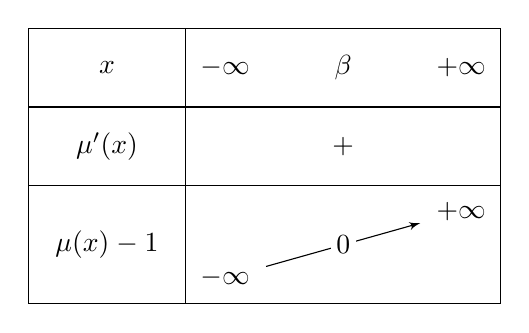
\begin{tikzpicture}
                  \tkzTabInit{$x$ /1, $\mu'(x)$ /1, $\mu(x)-1$ /1.5} {$-\infty$ , $+\infty$}
                  \tkzTabLine{, +,}
                  \tkzTabVar{-/$-\infty$, +/ $+\infty$}
                  \tkzTabVal{1}{2}{0.5}{$\beta$}{0} % On place 0, son antécédent est pi / 2.
              \end{tikzpicture}
          \end{center}
          \begin{itemize}
              \item $\forall x \in ]-\infty ; \beta[$, $\mu(x)-1 < 0 $
              \item $\forall x \in ]-\infty ; \beta[$, $\mu(x)-1 > 0 $
          \end{itemize}
\end{itemize}

\subsection*{Partie B}

La fonction $f$ est définie par :

\[
    f(x) =
    \begin{cases}
        \frac{2(x^3+1)}{x^2+1}, & \text{si } x < 1    \\[10pt]
        1 + \sqrt{2x -1},       & \text{si } x \geq 1
    \end{cases}
\]

\begin{enumerate}
    \item Montrer que $Df=\mathbb{R}$
          \[\text{Posons }
              f(x) =
              \begin{cases}
                  f_1(x), & \text{si } x < 1    \\[10pt]
                  f_2(x), & \text{si } x \geq 1
              \end{cases}
          \]
          \begin{itemize}
              \item[*] \( f_1 \) existe si \( x^2 + 1 \neq 0 \) et \( x < 1 \).

                  \( x \in \mathbb{R} \) et \( x < 1 \)

                  \( D_1 = ]-\infty, 1[ \)

              \item[*] \( f_2 \) existe si \( 2x -1 \geq 0 \) et \( x \geq 1 \).

                  \( 2x - 1 \geq 0 \Rightarrow x \geq \frac{1}{2} \)

                  \( x \geq \frac{1}{2} \) et \( x \geq 1 \)

                  \( x \in \left[ \frac{1}{2}, +\infty \right[ \text{ et } x\in[1, +\infty [ \)

                  \( x\in\left( \left[ \frac{1}{2}, +\infty \right[ \cap [1, +\infty [\right)  \)

                  \( x \in [1, +\infty[ \)

                  \(D_2 = [1, +\infty[\)
          \end{itemize}

          \(
          D_f = D_1 \cup D_2
          \)

          \(
          D_f = ]-\infty, 1[ \cup [1, +\infty[
          \)

          \(
          D_f = \mathbb{R}
          \)
    \item La continuité et la dérivabilité de \( f \) en 1

          \subsection*{Continuité}

          \underline{En \( 1^- \)} :

          \(
          f(x) = f_1(x) = \frac{2(x^3+1)}{x^2+1}
          \)

          \( \begin{aligned}
              \lim\limits_{x \to 1^-} f(x) & = \lim\limits_{x \to 1^-} \frac{2(x^3+1)}{x^2+1} \\
              = 2
          \end{aligned} \)

          \( \text{donc } \lim\limits_{x \to 1^-} f(x) = 2 \)

          \bigskip

          \underline{En \( 1^+ \)} :

          \( f(x) = f_2(x) = 1 + \sqrt{2x -1} \)

          \( \begin{aligned}
              \lim\limits_{x \to 1^+} f(x) & = \lim\limits_{x \to 1^+} 1 + \sqrt{2x -1} \\
                                           & = 2
          \end{aligned} \)

          \(  \text{donc } \lim\limits_{x \to 1^+} f(x) = 2 \)

          Comme
          \[
              \lim\limits_{x \to 1^-} f(x) = \lim\limits_{x \to 1^+} f(x) = f(1)
          \]
          donc \( f \) est continue en \( 1 \).

          \bigskip

          \underline{\textbf{Dérivabilité}}

          \underline{En \( 1^- \)}

          \(
          \begin{aligned}
              \lim\limits_{x \to 1^-} \frac{f(x) - f(1)}{x - 1} & = \lim\limits_{x \to 1^-} \frac{\frac{2(x^3+1)}{x^2+1} -2}{x-1}   \\
                                                                & = \lim\limits_{x \to 1^-} \frac{2x^3 +2 - 2x^2 - 2}{(x^2+1)(x-1)} \\
                                                                & = \lim\limits_{x \to 1^-} \frac{2x^3 - 2x^2}{(x^2+1)(x-1)}        \\
                                                                & = \lim\limits_{x \to 1^-} \frac{2x^2 (x-1)}{(x^2+1)(x-1)}         \\
                                                                & = \lim\limits_{x \to 1^-} \frac{2x^2}{(x^2+1)}                    \\
                                                                & = 1
          \end{aligned}
          \)

          \[
              \begin{aligned}
                  \lim_{x \to 1} \frac{f(x) - f(1)}{x - 1} & = \lim_{x \to 1} \frac{2x^2}{x^2 + 1} \\
                                                           & = 1
              \end{aligned}
          \]

          \( \text{Donc,}
          \begin{aligned}
              \lim_{x \to 1} \frac{f(x) - f(1)}{x - 1} & = 1
          \end{aligned}
          \)

          \underline{En \( 1^+ \)} :

          \(
          \begin{aligned}
              \lim_{x \to 1^+} \frac{f(x) - f(1)}{x - 1} & = \lim_{x \to 1^+} \frac{1 + \sqrt{2x - 1} - 2}{x - 1}           \\
                                                         & = \lim_{x \to 1^+} \frac{\sqrt{2x - 1} - 1}{x - 1}               \\
                                                         & = \lim_{x \to 1^+} \frac{2x - 1 - 1}{(x - 1)(\sqrt{2x - 1} + 1)} \\
                                                         & = \lim_{x \to 1^+} \frac{2(x - 1)}{(x - 1)(\sqrt{2x - 1} + 1)}   \\
                                                         & = \lim_{x \to 1^+} \frac{2}{\sqrt{2x - 1} + 1}                   \\
                                                         & = 1
          \end{aligned}
          \)

          \( \text{Donc } \lim_{x \to 1^+} \frac{f(x) - f(1)}{x - 1} = 1 \)

          \[
              \text{Finalement } \lim_{x \to 1^-} \frac{f(x) - f(1)}{x - 1} = \lim_{x \to 1^+} \frac{f(x) - f(1)}{x - 1}
          \]

          \[
              \text{Donc } f \text{ est dérivable en } 1.
          \]
    \item Équation de la tangente  (T) à \( \mathcal{C}_{f} \) \text{ au point } A(1,2).
          \[
              (T) : y = f'(1)(x - 1) + f(1)
          \]

          \[
              y = (x - 1) + 2
          \]

          \[
              \text{Donc } (T) : y = x + 1
          \]
    \item Position de \( (\mathcal{C}_f) \) par rapport à \( (T) \).

          Pour ce faire, étudions le signe de \( f(x) - y \).

          \underline{Pour \( x < 1 \)}

          \(
          \begin{aligned}
              f(x) - y & = \frac{2(x^3 + 1)}{x^2 + 1} - (x + 1)           \\
                       & = \frac{2(x^3 + 1) - (x + 1)(x^2 + 1)}{x^2 + 1}  \\
                       & = \frac{2x^3 + 2 - (x^3 + x + x^2 + 1)}{x^2 + 1} \\
                       & = \frac{2x^3 + 2 - x^3 - x^2 - x - 1}{x^2 + 1}   \\
                       & = \frac{x^3 - x^2 - x + 1}{x^2 + 1}
          \end{aligned}
          \)

          \(
          f(x) - y = \frac{x^3 - x^2 - x + 1}{x^2 + 1}
          \)

          \text{Le signe dépend du numérateur, que nous étudions avec la méthode de Horner :}

          \[
              \begin{array}{r|r|r|r|r|}
                  \hline
                    & 1 & -1 & -1 & 1 \\
                  \hline
                  1 & 1 & 0  & -1 & 0 \\
                  \hline
                    & 1 & 0  & -1 & 0 \\
                  \hline
              \end{array}
          \]

          \text{On obtient la factorisation :}

          \(
          \begin{aligned}
              x^3 - x^2 - x - 1 & = (x - 1)(x^2 - 1)      \\
                                & = (x - 1)(x - 1)(x + 1) \\
                                & = (x + 1)(x - 1)^{2}
          \end{aligned}
          \)

          \(
          \text{Donc } f(x) - y = \frac{(x + 1)(x - 1)^{2}}{x^2 + 1}
          \)

          \(
          \text{Si } x < -1, f(x) - y < 0 \text{ donc } (\mathcal{T}) \text{ est au-dessus de } (\mathcal{C}_f)
          \)

          \(
          \text{Si } x \in ]-1, 1[, f(x) - y > 0 \text{ donc } (\mathcal{C}_f) \text{ est au-dessus de } (\mathcal{T})
          \)

          \underline{Pour \( x > 1 \)}

          \(
          \begin{aligned}
              f(x) - y & = 1 + \sqrt{2x - 1} - (x + 1) \\
                       & = \sqrt{2x - 1} - x
          \end{aligned}
          \)

          \(
          \text{Supposons que } \sqrt{2x - 1} - x < 0
          \)

          \(
          \begin{aligned}
              \sqrt{2x - 1} < x
               & \Leftrightarrow
              \begin{cases}
                  x > 0      \\
                  2x - 1 > 0 \\
                  2x - 1 < x^2
              \end{cases}       \\
               & \Leftrightarrow
              \begin{cases}
                  x > 0      \\
                  2x - 1 > 0 \\
                  x^2 - 2x + 1>0
              \end{cases}
          \end{aligned}
          \)

          \(
          \text{Posons}
          \begin{cases}
              x > 0      \\
              2x - 1 > 0 \\
              x^2 - 2x + 1>0
          \end{cases}
          \)

          \(
          \begin{aligned}
              \begin{cases}
                  x = 0      \\
                  2x - 1 = 0 \\
                  x^2 - 2x + 1 = 0
              \end{cases}
               & \Leftrightarrow
              \begin{cases}
                  x = 0         \\
                  x=\frac{1}{2} \\
                  x = 1
              \end{cases}
          \end{aligned}
          \)

          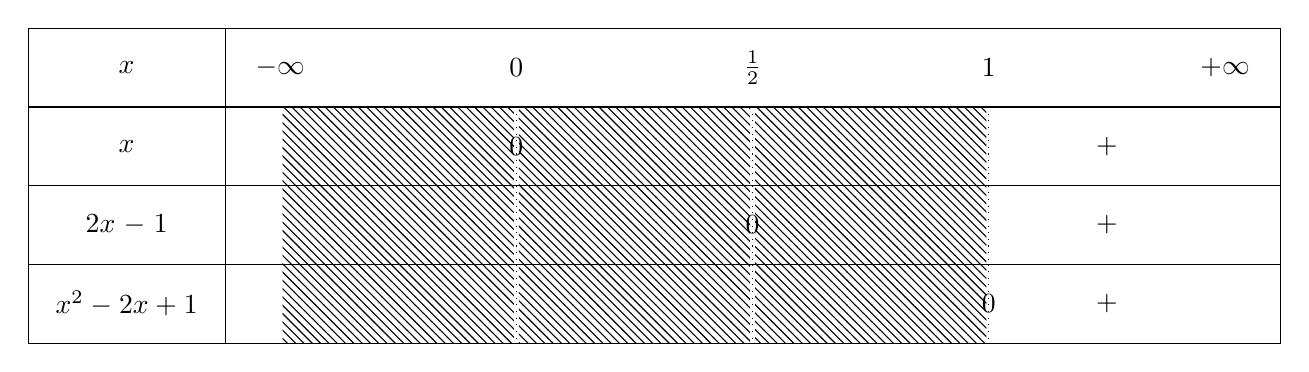
\begin{tikzpicture}
              \tkzTabInit[lgt = 2.5, espcl = 3, deltacl = 0.7]%
              {$x$ / 1 , $x$ / 1 , $2x - 1$ / 1 , $x^2 - 2x + 1$ / 1}%
              {$-\infty$, $0$, $\frac{1}{2}$, $1$, $+\infty$}
              \tkzTabLine{,h,z,h,t,h,t,+,}
              \tkzTabLine{,h,t,h,z,h,t,+,}
              \tkzTabLine{,h,t,h,t,h,z,+,}
          \end{tikzpicture}

          \(
          \text{Donc pour que } \sqrt{2x - 1} - x < 0, \text{ il faut que } x \geq 1
          \)

          \(
          \text{Donc si } x \geq 1 \text{ alors } f(x) - y < 0
          \)

          \(
          \text{D'où si } x \geq 1 \text{ alors } (\mathcal{T}) \text{ est au-dessus de } (\mathcal{C}_f)
          \)

    \item
          \begin{enumerate}
              \item Montrons que\( \forall x \in ]-\infty,1[, f'(x) =   \frac{2x\left[u(x)-1\right]}{(x^2+1)^2}  \)

                    \(\forall x \in ]-\infty,1[, \quad f(x) = \frac{2(x^3+1)}{x^2+1}\)

                    \(
                    \begin{aligned}
                        f'(x) & = \frac{2x \left( 3x^2 (x^2+1) - 2x (x^3+1) \right)}{(x^2+1)^2} \\[10pt]
                              & = \frac{2x \left[ 3x (x^2+1) - 2x (x^3+1) \right]}{(x^2+1)^2}   \\[10pt]
                              & = \frac{2x \left[ 3x^3 + 3x - 2x^4 - 2x \right]}{(x^2+1)^2}     \\[10pt]
                              & = \frac{2x \left[ x^3 + 3x - 1 -1 \right]}{(x^2+1)^2}
                    \end{aligned}
                    \)


                    \( \forall x \in ]-\infty,1[, f'(x) =   \frac{2x\left[u(x)-1\right]}{(x^2+1)^2} \quad \text{cqfd.} \)

              \item  Calculons \( f'(x) \) pour \( x \in [1,+\infty[ \)

                    \[
                        f(x) = 1 + \sqrt{2x - 1}
                    \]

                    \[
                        f'(x) = \frac{2}{2\sqrt{2x - 1}}
                    \]

                    \[
                        = \frac{1}{\sqrt{2x - 1}}
                    \]

                    \[
                        \text{Donc } \forall x \in [1,+\infty[, \quad f'(x) = \frac{1}{\sqrt{2x - 1}}
                    \]
              \item  Le signe de \( f'(x) \) sur \( \mathbb{R} \)

                    \textcolor{red}{ Sur \( ]-\infty; 1[, f'(x) = \frac{1}{\sqrt{2x - 1}} \)}

                    Le signe de \( f(x) \) dépend du numérateur.

                    D'après la réponse à la question d) de la partie A, on a :
                    \(
                    \begin{cases}
                        \forall x \in ] - \infty, \beta [ , \mu(x) - 1 < 0 \\
                            \forall x \in ] \beta, + \infty [, \mu(x) - 1 > 0
                    \end{cases}
                    \)

                    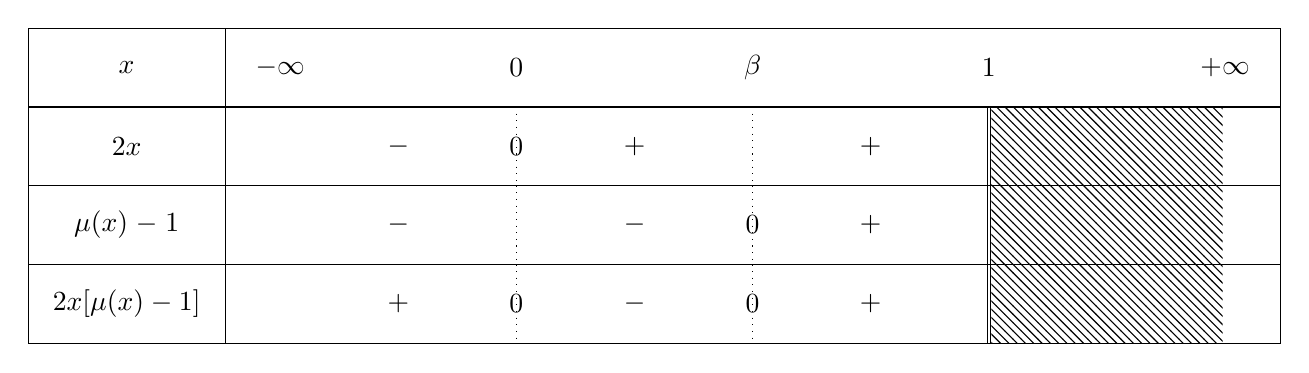
\begin{tikzpicture}
                        \tkzTabInit[lgt = 2.5, espcl = 3, deltacl = 0.7]%
                        {$x$ / 1 , $2x$ / 1 , $\mu(x) - 1$ / 1 , $2x[\mu(x) - 1]$ / 1}%
                        {$-\infty$, $0$, $\beta$, $1$, $+\infty$}
                        \tkzTabLine{,-,z,+,t,+,d,h,}
                        \tkzTabLine{,-,t,-,z,+,d,h,}
                        \tkzTabLine{,+,z,-,z,+,d,h,}
                    \end{tikzpicture}

                    Finalement
                    \begin{itemize}
                        \item Si \( \, x \in ] -\infty, 0 [ \cup ] \beta, 1 [ , f'(x   ) > 0\) \\
                              donc \( f \) est croissante.
                        \item Si \( \, x \in ] 0, \beta [ , f'(x) < 0\) \\
                              donc \( f \) est décroissante.
                    \end{itemize}
                    \textcolor{red}{Sur \( [1, +\infty[, f'(x) = \frac{1}{\sqrt{2x - 1}}\)}

                    \( \forall x \in |1, +\infty[, \quad f'(x) > 0 \)

                    Donc \( f \) est croissante sur \( |1, +\infty[ \).
              \item Tableau de variation
                    \begin{center}
                        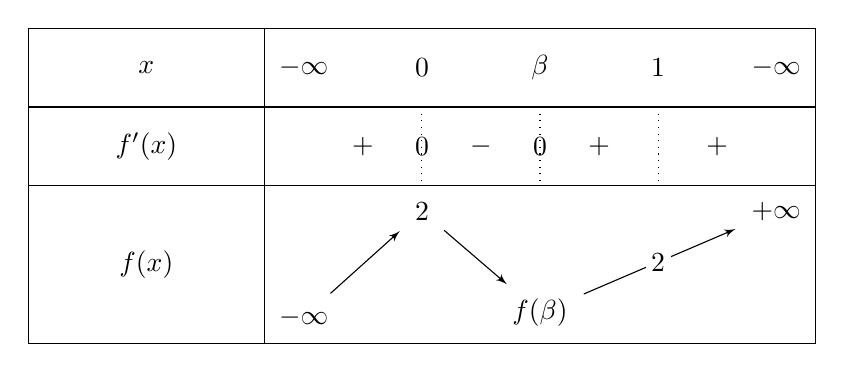
\begin{tikzpicture}
                            \tkzTabInit[lgt=3,espcl=1.5]
                            {$x$ / 1 , $f'(x)$ / 1, $f(x)$ / 2 }
                            {$-\infty$, $0$, $\beta$, 1, $-\infty$}
                            \tkzTabLine
                            {, +, z ,  -  , z , + ,t,+,}
                            \tkzTabVar
                            { -/$-\infty$ , +/$2$, -/$f(\beta)$, R/, +/$+\infty$}
                            \tkzTabIma{3}{5}{4}{2}
                        \end{tikzpicture}
                    \end{center}
                    Limites aux bornes de \( D_f = \mathbb{R} \)

                    \underline{En \( -\infty \) :}

                    \(
                    \begin{aligned}
                        \lim_{x \to -\infty} f(x) & = \lim_{x \to -\infty} \frac{2(x^3 + 1)}{x^2 + 1} \\
                                                  & = \lim_{x \to -\infty} \frac{2x^3 + 2}{x^2 + 1}   \\
                                                  & = \lim_{x \to -\infty} \frac{2x^3}{x^2}           \\
                                                  & = \lim_{x \to -\infty} 2x                         \\
                                                  & = -\infty
                    \end{aligned}
                    \)

                    \underline{En \( +\infty \) :}

                    \(
                    \begin{aligned}
                        \lim_{x \to +\infty} f(x) & = \lim_{x \to +\infty} \left( 1 + \sqrt{2x - 1} \right) \\
                                                  & = +\infty
                    \end{aligned}
                    \)

          \end{enumerate}

    \item
          \begin{enumerate}
              \item Les Bandes Asymptotiques

                    \underline{En \( -\infty \) :}

                    Puisque
                    \(
                    \lim_{x \to -\infty} f(x) = -\infty,
                    \)
                    cherchons
                    \(
                    \lim_{x \to -\infty} \frac{f(x)}{x}.
                    \)

                    \(
                    \begin{aligned}
                        \lim_{x \to -\infty} \frac{f(x)}{x} & = \lim_{x \to -\infty} \frac{\frac{2(x^3 + 1)}{x^2 + 1}}{x} \\
                                                            & = \lim_{x \to -\infty} \frac{2x^3 + 2}{x^3 + x}             \\
                                                            & = \lim_{x \to -\infty} \frac{2x^3}{x^3}                     \\
                                                            & = 2.
                    \end{aligned}
                    \)

                    Ainsi,
                    \(
                    \lim_{x \to -\infty} \frac{f(x)}{x} = 2.
                    \)
                    Donc, cherchons
                    \(
                    \lim_{x \to -\infty} \left[ f(x) - 2x \right].
                    \)

                    \[
                        \begin{aligned}
                            \lim_{x \to -\infty} \left( f(x) - 2x \right) & = \lim_{x \to -\infty} \left( \frac{2(x^3 + 1)}{x^2 + 1} - 2x \right) \\
                                                                          & = \lim_{x \to -\infty} \frac{2x^3 + 2 - 2x(x^2 + 1)}{x^2 + 1}         \\
                                                                          & = \lim_{x \to -\infty} \frac{2x^3 + 2 - 2x^3 - 2x}{x^2 + 1}           \\
                                                                          & = \lim_{x \to -\infty} \frac{-2x + 2}{x^2 + 1}                        \\
                                                                          & = \lim_{x \to -\infty} \frac{-2x}{x^2}                                \\
                                                                          & = \lim_{x \to -\infty} \frac{-2}{x}                                   \\
                                                                          & = 0.
                        \end{aligned}
                    \]

                    Ainsi, \( (\mathcal{C}) \) admet une branche parabolique de direction \( y = 2x \).

                    \underline{En \( +\infty \) :}

                    Puisque

                    \(
                    \lim_{x \to +\infty} f(x) = +\infty,
                    \)

                    cherchons
                    \(
                    \lim_{x \to +\infty} \frac{f(x)}{x}.
                    \)

                    \(
                    \begin{aligned}
                        \lim_{x \to +\infty} \frac{f(x)}{x} & = \lim_{x \to +\infty} \frac{1 + \sqrt{2x - 1}}{x}                                   \\
                                                            & = \lim_{x \to +\infty} \frac{1 - (2x - 1)}{x \left[ 1 - \sqrt{2x - 1} \right]}       \\
                                                            & = \lim_{x \to +\infty} \frac{2(1 - x)}{x \sqrt{1 - \frac{2}{2x - 1}}}                \\
                                                            & = \lim_{x \to +\infty} \left( \frac{x - 1}{x} \times \frac{2}{1-\sqrt{2x-1}} \right) \\
                                                            & = \frac{1}{1} \times \frac{1}{\infty}                                                \\
                                                            & = 0.
                    \end{aligned}
                    \)

                    Ainsi, \( (\mathcal{C}) \) admet une branche parabolique de direction \( Ox \).
              \item La courbe \( (\mathcal{C}) \)
                    \begin{center}
                        \begin{figure}[H]% Forcer l'image à cet endroit
                            \centering
                            \includegraphics[width=0.8\textwidth]{/home/pathegobelba/Documents/LatexCodes/EvaluationTS2/build/curveExam1.png}
                            \caption{Courbe de (Cf)}
                            \label{fig:monimage}
                        \end{figure}
                    \end{center}
                    \href{https://www.geogebra.org/classic/tezwefad}{Clique ici pour voir la figure sur géogébra}
          \end{enumerate}
    \item
          \begin{enumerate}
              \item $g$ est continue et croissante sur $[1;\infty[$ donc réalise une bijection de $[1;\infty[$ vers $J=[2;\infty[$
              \item Comme $\forall x \in [1;\infty[, g'(x)\neq 0$ donc donc $g^{-1}$ estn dérivable sur $J$ et a même sens de variation que $g$ donc croissante aussi.
              \item Courbe $g^{-1}$
                    \begin{center}
                        \begin{figure}[H]% Forcer l'image à cet endroit
                            \centering
                            \includegraphics[width=0.8\textwidth]{/home/pathegobelba/Documents/LatexCodes/EvaluationTS2/build/CourbeReciproqueProblemeDeremplacementCompo1.png}
                            \caption{Courbe de (Cf)}
                            \label{fig:monimage}
                        \end{figure}
                    \end{center}
                    \href{https://www.geogebra.org/m/enjrqsgy}{Clique ici pour voir la figure sur géogébra}
          \end{enumerate}
\end{enumerate}

\end{document}